\documentclass[12pt]{article}

\usepackage{amsmath, amssymb, amsthm, graphicx, fancyhdr, textcomp, enumerate, diagbox, tcolorbox, esvect, tikz, adjustbox}

\graphicspath{{./images/}}

\usepackage{halloweenmath, tikzsymbols}

\newcommand{\R}{\mathbb{R}}
\newcommand{\Z}{\mathbb{Z}}
\newcommand{\C}{\mathbb{C}}
\newcommand{\N}{\mathbb{N}}
\newcommand{\Q}{\mathbb{Q}}
\newcommand{\Arg}{\mbox{Arg}}
\newcommand{\Log}{\mbox{Log}}

%geometry/topology
\newcommand{\bndry}{\partial}


\newcommand{\infsum}{\sum_{n = 1}^{\infty}}
\newcommand{\pf}{\fbox{proof}}
\newcommand{\cor}{\fbox{corollary}}

\theoremstyle{definition}

\newtheorem*{definition}{Definition}
\newtheorem{lemma}{Lemma}
\newtheorem{theorem}{Theorem}
\newtheorem{corollary}{Corollary}
\newtheorem{proposition}{Proposition}
\newtheorem{remark}{Remark}
\newtheorem{conjecture}{Conjecture}
\newtheorem{example}{Example}

\newcommand{\inv}[1]{#1^{-1}}

\title{Modern Geometry}
\author{August}

\begin{document}

\maketitle

\section{Problem 4.7}

Draw the Voronoi region for this point set:

\[ S = \{(1,3),(1,9),(1,11),(3,6),(4,9),(6,6)\} \]

Here it is!


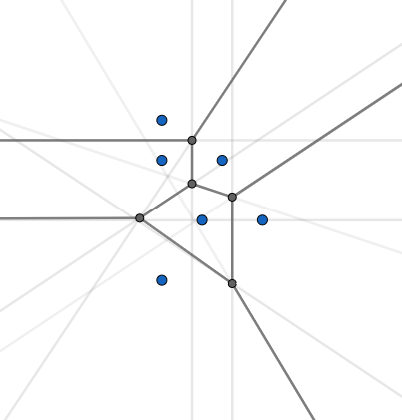
\includegraphics[scale=1]{voronoi_4_7.png} 

Drawn using trusty Geogebra and perpendicular bisectors!

\section{Problem 4.14}

For this problem I'll "need" a "technical" lemma (even though I'll hand-wave other things). I'll have to prove the
\begin{lemma}
Let $p_1p_2p_3$ be a triangle, and let $p$ be interior to it. Then the half-plane of the perpendicular bisector of $p_1p$ ($\ell$) which contains $p$ also contains one of $p_2,p_3$.
\end{lemma}

\begin{proof}
To see this, notice that $p_1p$, after crossing through $p$, also must cross an edge of the triangle. Moreover, this edge cannot be $p_1$ (for the edges $p_1p_i$ are convex, the line crosses through $p$, and $p$ is not in $p$). Therefore this edge is the only edge which is not adjacent to $p$: $p_2p_3$. Moreover, the perpendicular bisector $\ell$ crosses through $p$ (an interior point of the triangle), therefore it must cross the boundary of the triangle. Here there are two cases. Either it crosses $p_2p_3$ or it doesn't. If it crosses $p_2p_3$, then it also crosses at another point, and by a similar convexness argument about edges, this cannot be the same side of the triangle. If it doesn't cross $p_2p_3$, then it certainly crosses somewhere else!\\

Without loss of generality, suppose $\ell$ crosses the side $p_1p_2$. I claim that $p_3$ is on the same side of $p$ of $\ell$. 

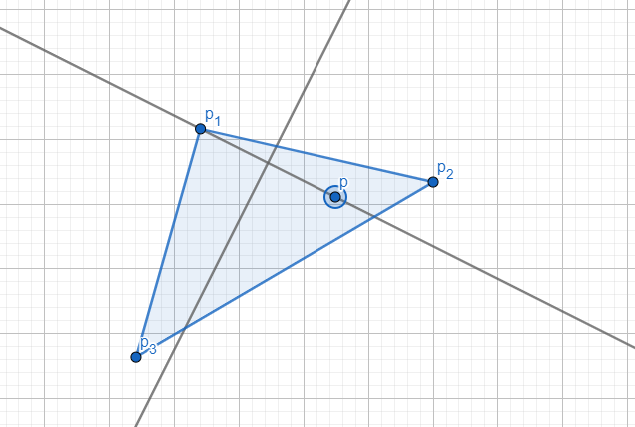
\includegraphics[scale=1]{techincal_lemma.png} 
\end{proof}

\begin{proposition}

Let $S$ be a point set. The voronoi region of a point $p\in S$ is unbounded if and only if $p$ is a hull vertex.

\end{proposition}

\begin{proof}
First suppose that $p$ is not a hull vertex. Then it is in the interior of the convex hull. The convex hull forms a convex polygon whose vertices are the hull vertices, and polygons can be triangulated. Pick some triangulation $T$. If $p$ lies on the edge of a triangle, flip the edge upon which it lies through a sequence of flips (this is possible because the convex hull is a convex polygon) until $p$ is on the interior of one of the triangles. 

Let $p_1p_2p_3$ be the triangle which contains $p$, where $p_i$ are hull vertices. Now consider the intersection of the half planes $H(p,p_i)$ with $i = 1,2,3$. I claim that this intersection is a triangle which contains $p$. This can be seen from noting that no three of $p_i$ are parallel, and the lines which give us these half planes are perpendicular to these lines. Therefore none of these lines are pairwise parallel. Therefore the lines (which are the perpendicular bisectors) intersect at three points. These three points form a triangle, formed by intersecting the half planes which contain the other vertices of the triangle. By the lemma, these half planes are the ones which also contain $p$, so $p$ is contained within this triangle, which is the intersection of half planes containing $p$. But the voronoi region of $p$ is the intersection of such half planes, therefore the voronoi region is contained within the triangle we have constructed. Since this triangle is a bounded region, it follows that the voronoi region of $p$ is as well. 


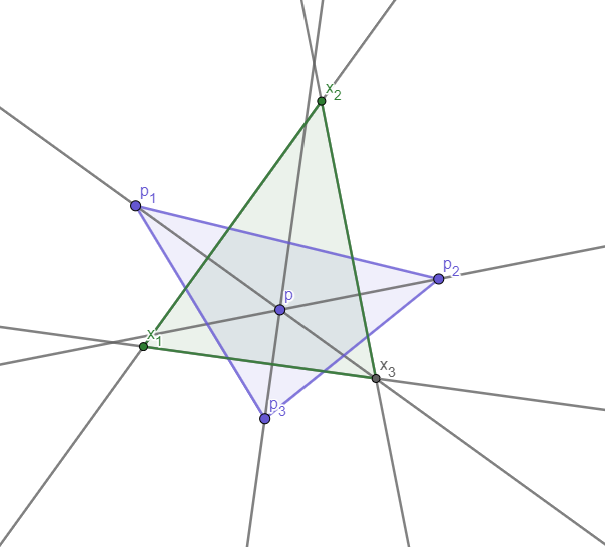
\includegraphics[scale=1]{bounded_region_triangle.png} 

Suppose that the Voronoi region of $p$ is bounded, yet $p$ is a hull vertex of $S$. Since $p$ is a hull vertex of $S$, it is possible to draw a tangent line $\ell$ at $p$. Let a line not parallel to $\ell$ cross through $p$, let this line be $m$. Then half of $m$ is on the side of $\ell$ which does not contain $S$. Moreover, since the Voronoi region of $p$ is bounded, it follows that both sides of $m$ cross an edge of the Voronoi region, so let $x$ be the crossing with the edge $e$ on the side of $\ell$ opposite $S$. Extend $e$ as a line. If $e$ is parallel to $\ell$, then adjust $\ell$ so that it isn't and start all over again (the possibilities for $\ell$ are infinite, the possibilities for $e$ are finite for the edges are determined by $S$ which is finite). Since $\ell$ is not parallel to $e$, it follows that $\ell$ and $e$ cross at some point $y$. Form the triangle $pxy$. It is a fact that the perpendicular line from any vertex of a triangle to any of its edges crosses the interior of the triangle, therefore the perpendicular line to $e$ which crosses through $ p $ is partly contained within $pxy$. But the edges of the voronoi region of $p$ are the perpendicular bisectors of points in $S$ with $p$, therefore extending past $e$ we find that there must be a point $q\in S$ so that $e$ is the perpendicular bisector of $p$ and $q$. But since $pq$ extends further into the side of $\ell$ which is opposite $S$, we have a point of $S$ other than $p$ which is on the side of $\ell$ which doesn't contain any points of $S$ other than $p$. This is a contradiction.

\end{proof}

\section{4.15}

\begin{proposition}
The average number of vertices per veronoi region in a veronoi diagram is less than $6$, for $n> 3$ sites.
\end{proposition}

\begin{proof}
Assume general position. Clearly if we have three sites, we can have only one vertex for each cell, which is pretty darn less than $6$. Now suppose that for $n$ vertices we have that the average number of vertices per cell is less than $6$. If we let $X_n$ be the sum over each region over the number of vertices of those regions. Then $\overline{V}_n = X_n/n < 6$. Now add a new vertex. Adding a new vertex, we can have at most $2$ vertices. This is because, by the formula of the textbook, for the original veronoi diagram we have $V_0 = 2n - 5$ vertices, whereas in the new veronoi diagram we have $V_1 = 2(n + 1)- 5$ vertices. Hence $\Delta V = V_1 - V_0 = 2$, so we have gained exactly two vertices in adding one new vertex. Since we are in general position, there are exactly $3(2) = 6 $ new vertices in the sum over cells.  Hence \[\overline{V}_{n+1} = (X_n + 6) /(n+1) = \frac{(X_n + 6) (1/n)}{(n+1)(1/n)} =  \frac{X_n / n + 6/n}{1 + \frac{1}{n}} < 6\frac{1 + \frac{1}{n}}{1 + \frac{1}{n}} = 6\]
This completes the proof.
\end{proof}

\section{(Order 2 Voronoi diagrams)}
To prove the 
\begin{theorem}
Given a point set $S$, and $p,q\in S$, $V_2(p,q)$ is non-empty if and only if $V_1(p)$ and $V_1(q)$ share a boundary.  
\end{theorem}

we need the 
\begin{lemma}
$V_2(p,q) \subset V_1(p)\cup V_1(q)$.
\end{lemma}

We can verify this with the

\begin{proof}

Let $x\in V_2(p,q)$. Then by definition of the voronoi diagram for any $r$ not $p$ or $q$, $d(x,r) \le d(x,p), d(x,q)$. By the trichotomy law, either $d(x,p) = d(x,q)$, $d(x,p) > d(x,q)$, or $d(x,p) < d(x,q)$. If $d(x,p) = d(x,q)$, $d(x,p)\le d(x,q)$, and also $d(x,p) \le d(x,r)$ for all the $r\ne q$ in $S$. By definition of the voronoi region, we have $x\in V_1(p)$. The case where $d(x,q) < d(x,p)$ and the other way around follow pretty much identically. In either case, we have that $x\in V_1(p)\cup V_1(q)$. 

\end{proof}

This is enough to prove the theorem.

\begin{proof}
First, suppose that $V_1(p)$ and $V_2(q)$ share a boundary point $x$. Then $x\in V_1(p)\cap V_2(q)$, hence $x$ is closest to both $p$ and $q$, as follows by definition of the voronoi region. As a result, $x\in V_2(p,q)$.\\

Now for the converse. We proceed by contradiction. Suppose that we have some $x\in V_2(p,q)$ while $V_1(p)$ and $V_1(q)$ are not neighbors. By our lemma, $x$ is in one of these cells. Without loss of generality, let us suppose $x\in V_1(p)$. Now draw the line segment $qx$. Since $q\in V_1(q)$, and since $x\not \in V_1(q)$, it follows that $qx$ crosses the boundary of $V_1(q)$ at some point $y$. Since the boundary consists of perpendicular bisectos between points in $S$, it follows that there exists some $r\in S$ such that $y$ is on the perpendicular bisector of $rq$. Moreover, since $V_1(p)$ and $V_2(q)
$ are not neighbors, it follows that $r\ne p$, or else part of this line would be a shared edge. Hence $x$ is on the other side of the line $rq$ than $q$, so $x$ is closer to $r$ than to $q$. As a result, $x$ is not in $V_2(p,q)$, but we have supposed it was. This is a contradiction, and it suffices to prove the converse.
 \end{proof}

This simple theorem gives us quite a bit of power in tranfering our problem to a better understood domain: voronoi diagrams. In fact, we have an upper bound for the number of edges in a Voronoi diagram. Moreoer, since the vertices of the Voronoi diagram have degree $3$ in general position, sharing a vertex implies sharing an edge. This proves the corollary

\begin{corollary}
For point sets in general position, the maximum number of non-empty order two veronoi regions with $n$ points is $3n-6$. Moreover, the non-empty order-two voronoi regions are in bijection with the edges of such a veronoi diagram.
\end{corollary}

If we are not in general position, we can have degree four vertices, which opens up the possibility of having neighboring Voronoi regions only through vertices. Nonetheless, with only 6 vertices, not having general position is unlikely to help much, as it generally reduces the number of shared boundaries in general. The only reason I mention this is that the proof of the corollary does rely on the vertices having degree 3.

Now we have a particular upper bound for the number of non-empty order two veronoi diagrams can be in a point set of six vertices. This is $ 3(6) - 6 = 12 $. We need only construct an example of such a point set, and here it is!

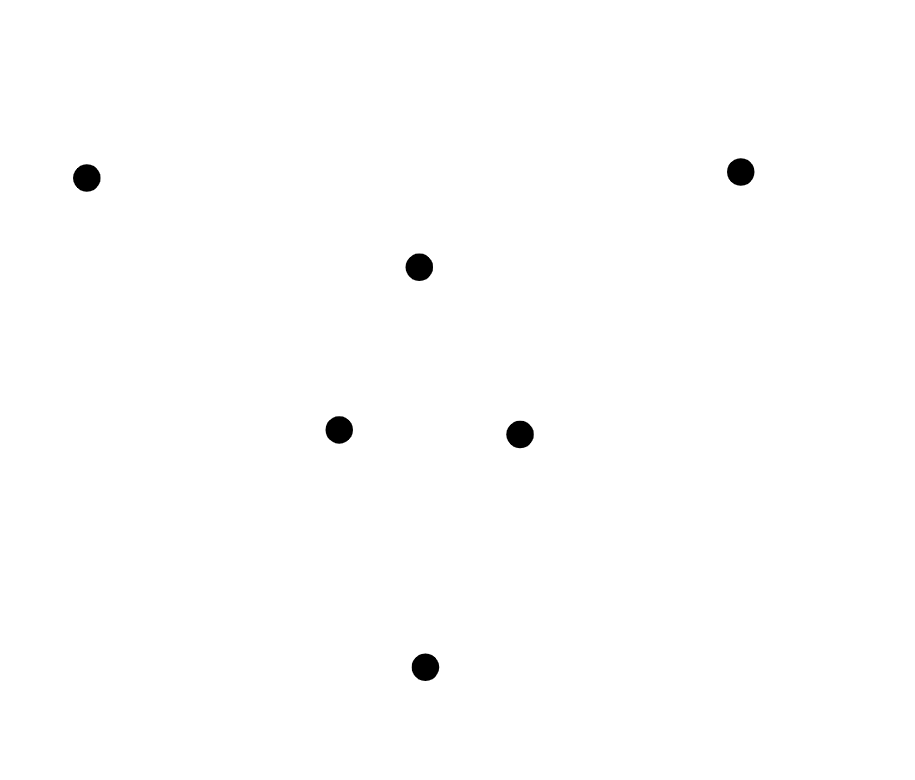
\includegraphics[scale=1]{point_set.png} 

This is the example, but it doesn't help us much until we see the Voronoi diagram, so let's see it.

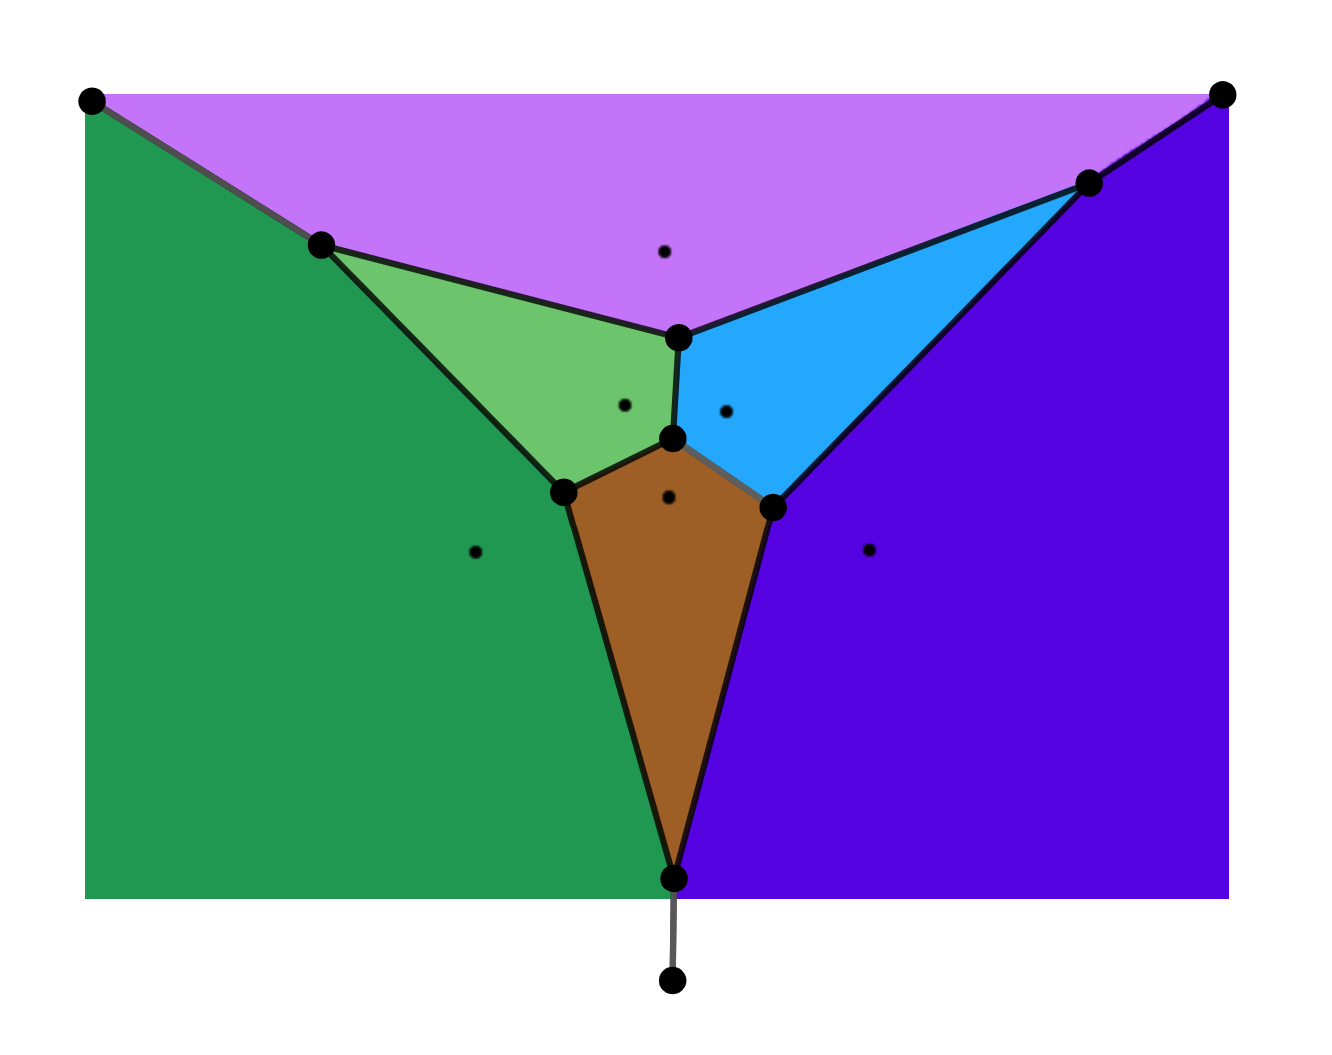
\includegraphics[scale=0.5]{second_order_voronoi.png} 

Notice each vertex has degree 3. As one who can count, it is clear that there are twelve vertices. Hence we have exactly as many vertices as we have twelve non-empty regions. As we showed, this is as good as we can get. \\


In my opinion, the beauty of this solution is that we don't know what the regions look like. We just know that they're there, through an abstract argument. Still, I \textit{guess} the assignment was to find and draw the maximum number of non-empty regions, so here goes I guess:

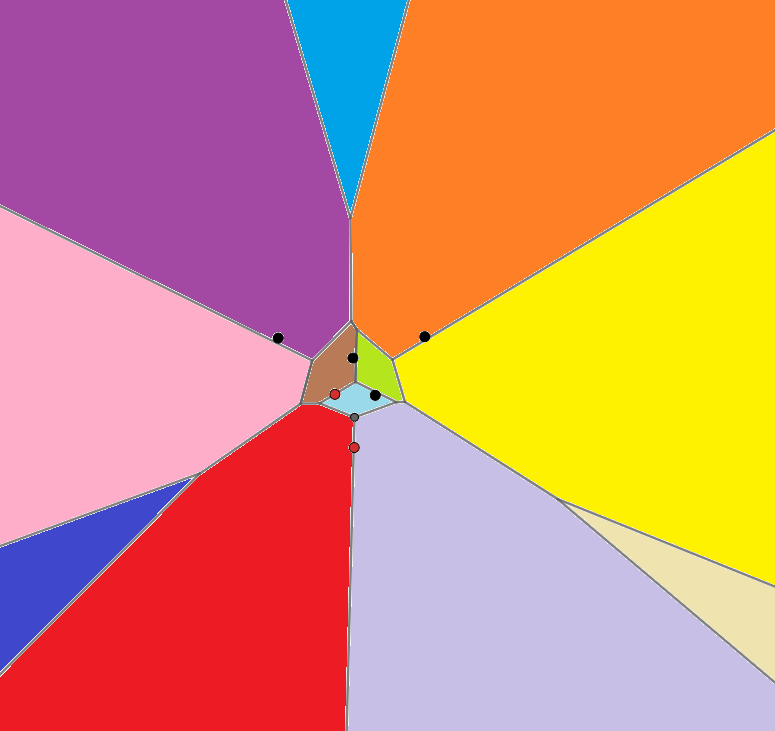
\includegraphics[scale=0.50]{Order_2_Voronoi.png} 

Given our discoveries, it is very easy to figure out the smallest possible amount we can get with four points. We can get exactly five non-empty regions, and no less. In any Voronoi diagram, there is at least one edge for each voronoi cell. The least we can get is by putting six of them collinear:

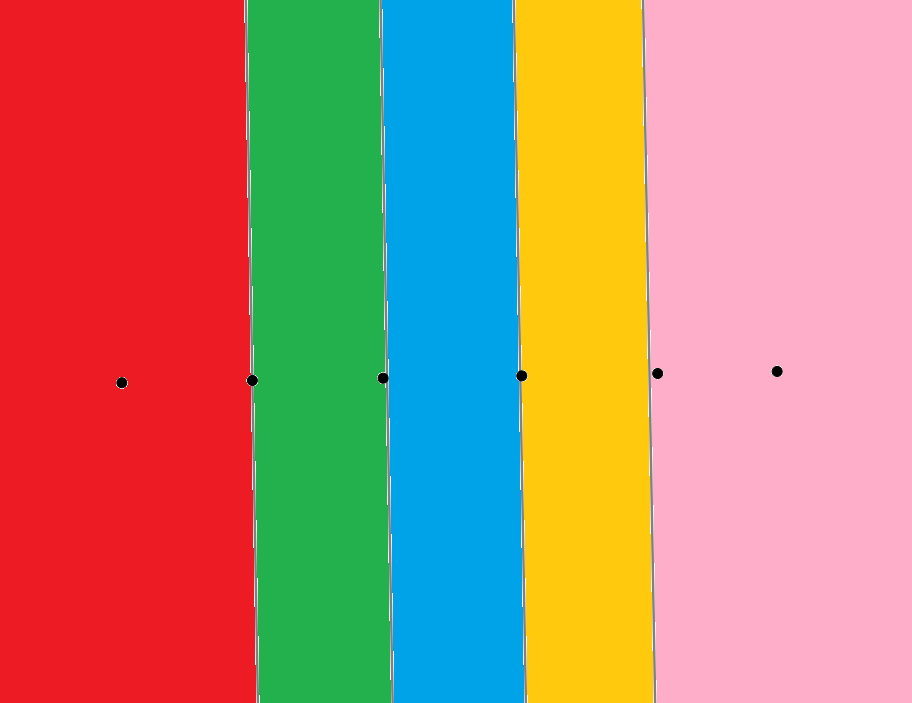
\includegraphics[scale=0.25]{smallest_order_2.png} 



\section{Problem (c)}

\begin{definition}

Given a point set $S\subset \R^2$ and a point $p$ in $S$, the farthest point region of $p$ is the set,

\[V_f(p) = \{x \in \R^2 : d(x,p ) \ge d(x,q) \forall q\in S\}\]
\end{definition}

\begin{proposition}
The farthest point region of $p$ is convex.
\end{proposition}
\begin{proof}
From this definition, it is clear that 
\[ V_f(p) = \bigcap_{q\ne p \in S} H'(p,q) \] where $H'(p,q) = \{x\in \R^2 : d(x,p) \ge d(x,q)\}$. We are simply adding one more requirement in the construction of the set. Recall that $H(p,q) = \{x\in \R^2 : d(x,p) \le d(x,q)\}$ was shown to be the half plane of the perpendicular bisector to $pq$ which contains $p$. The sets $ H'(p,q) $ simply have the inequality reversed: they are the half planes of the perpendicular bisectors of $pq$ which \textbf{don't} contain $p$. These are still half planes. The half planes are convex. Moreover, we have a proof from the textbook that the intersection of convex regions is convex. Hence the farthest point region of $p$ is convex.
\end{proof}

\section{ Taxicab Stuff }

Given two points, we can get at most three edges. Colliding one of these edges to add a third point, it is possible to have five more edges. Finally, adding another point, we find that we have five more edges. In total, we have thirteen, and this is the best we can do because we tried really hard to get there.

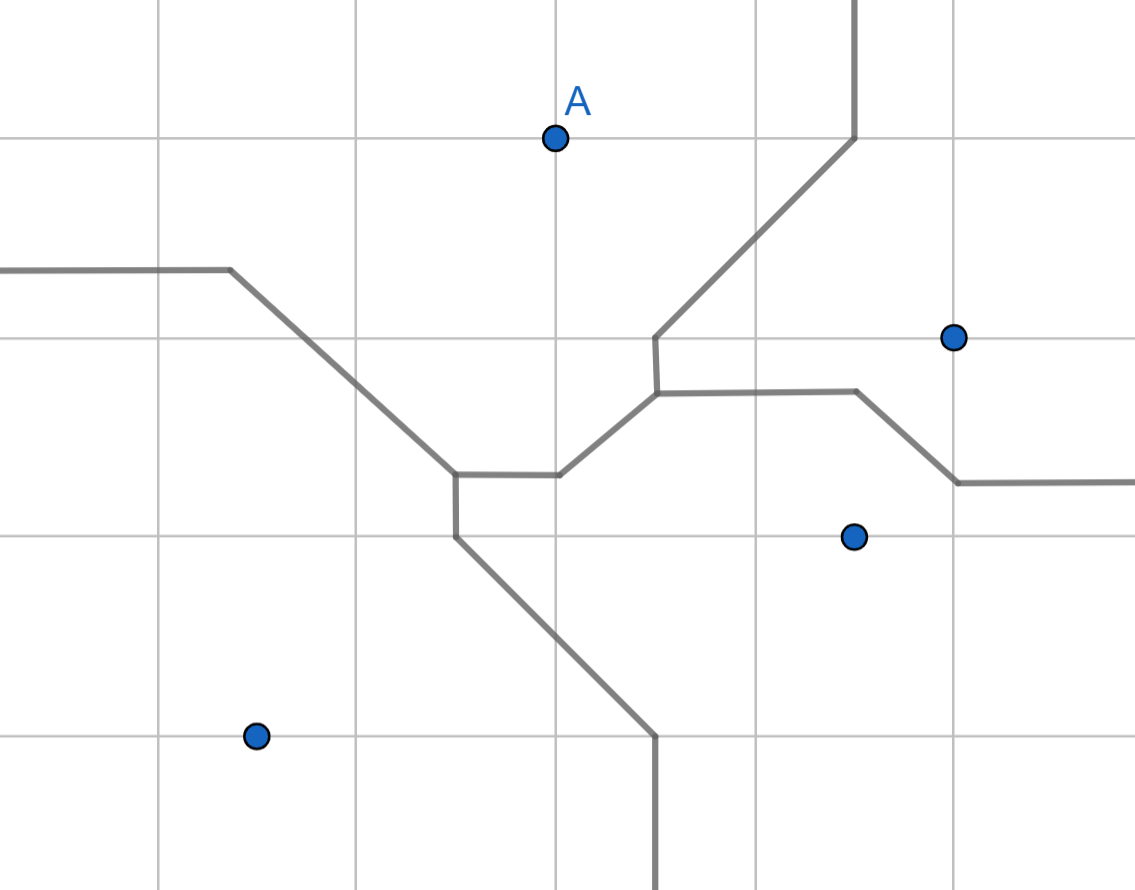
\includegraphics[scale=1]{taxicab.png} 

Noting that by considering congruent triangles we find that the taxicab region boundary between two two which have the same $y$ value is just the straight vertical line which bisects them, we find that the minimum number of edges is achieved like this:

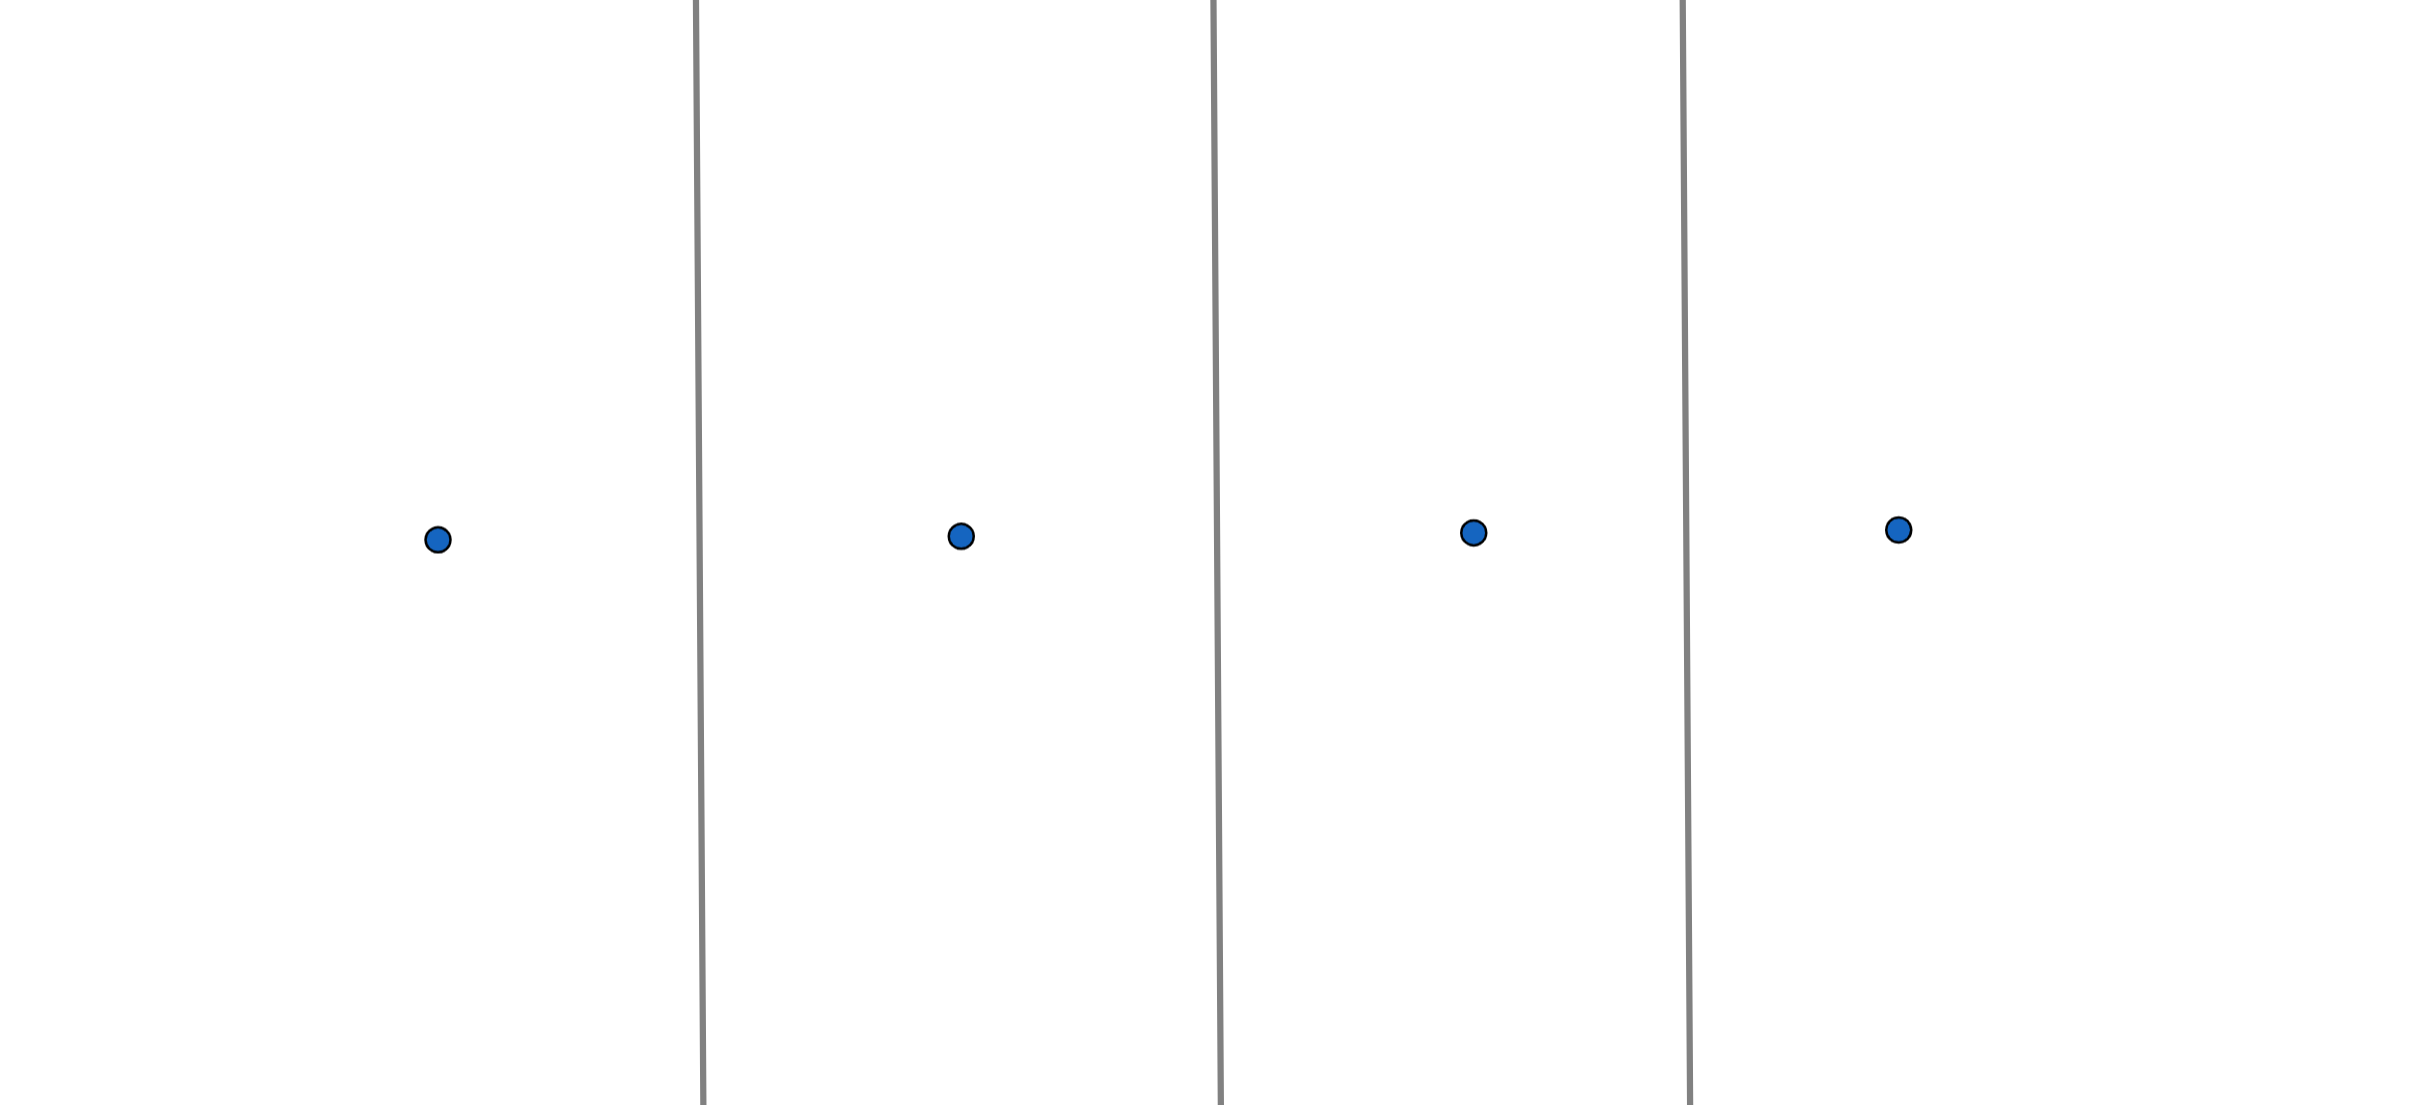
\includegraphics[scale=0.5]{smallest_taxicab.png} 


\end{document}